\documentclass[11pt,letterpaper]{article}
\usepackage[margin=1in]{geometry}
\usepackage{graphicx}
\usepackage{hyperref}
\usepackage{booktabs}
\usepackage{xcolor}
\usepackage{listings}

\graphicspath{{figures/}}

\lstset{
  basicstyle=\ttfamily\small,
  frame=single,
  breaklines=true,
  columns=fullflexible,
  backgroundcolor=\color{gray!8}
}

\hypersetup{colorlinks=true, urlcolor=blue, linkcolor=blue}

\title{CAT User and Administrator Manual\\[2pt]
  \large A shared human and AI workspace for discussing a codebase\\[16pt]
  
\includegraphics[width=0.13\textwidth]{mark.png}}
\author{Paul Fishwick and Claude Code}
\date{September 2026}

\begin{document}

\maketitle
\tableofcontents
\newpage

\section{Introduction}

CAT is a small chat workspace in which a research group discusses a specific
GitHub codebase, with AI agents participating as named members of the
conversation. It resembles Slack in shape---a sidebar of channels, a message
list, a composer---but it is deliberately much smaller, and it makes one
commitment Slack does not: a channel is bound to a repository, and the agents
in that channel can read it. The exception proves the rule: \texttt{\#general}
is bound to nothing, and is simply a room to talk in.

The system is designed for a group of fewer than twenty people. That constraint
is not incidental. It is what makes it reasonable to let every member read every
channel, to manage membership by adding rows to a table, and to run the whole
thing on free hosting.

A second constraint shapes it just as much: only some people may invoke an AI
agent. Everyone can read, everyone can talk, but summoning an agent spends money
against an API key, and that permission is granted individually. Hiding a button
would not be a control, so the check lives on the server, in the one place the
key exists.

\begin{figure}[h]
\centering
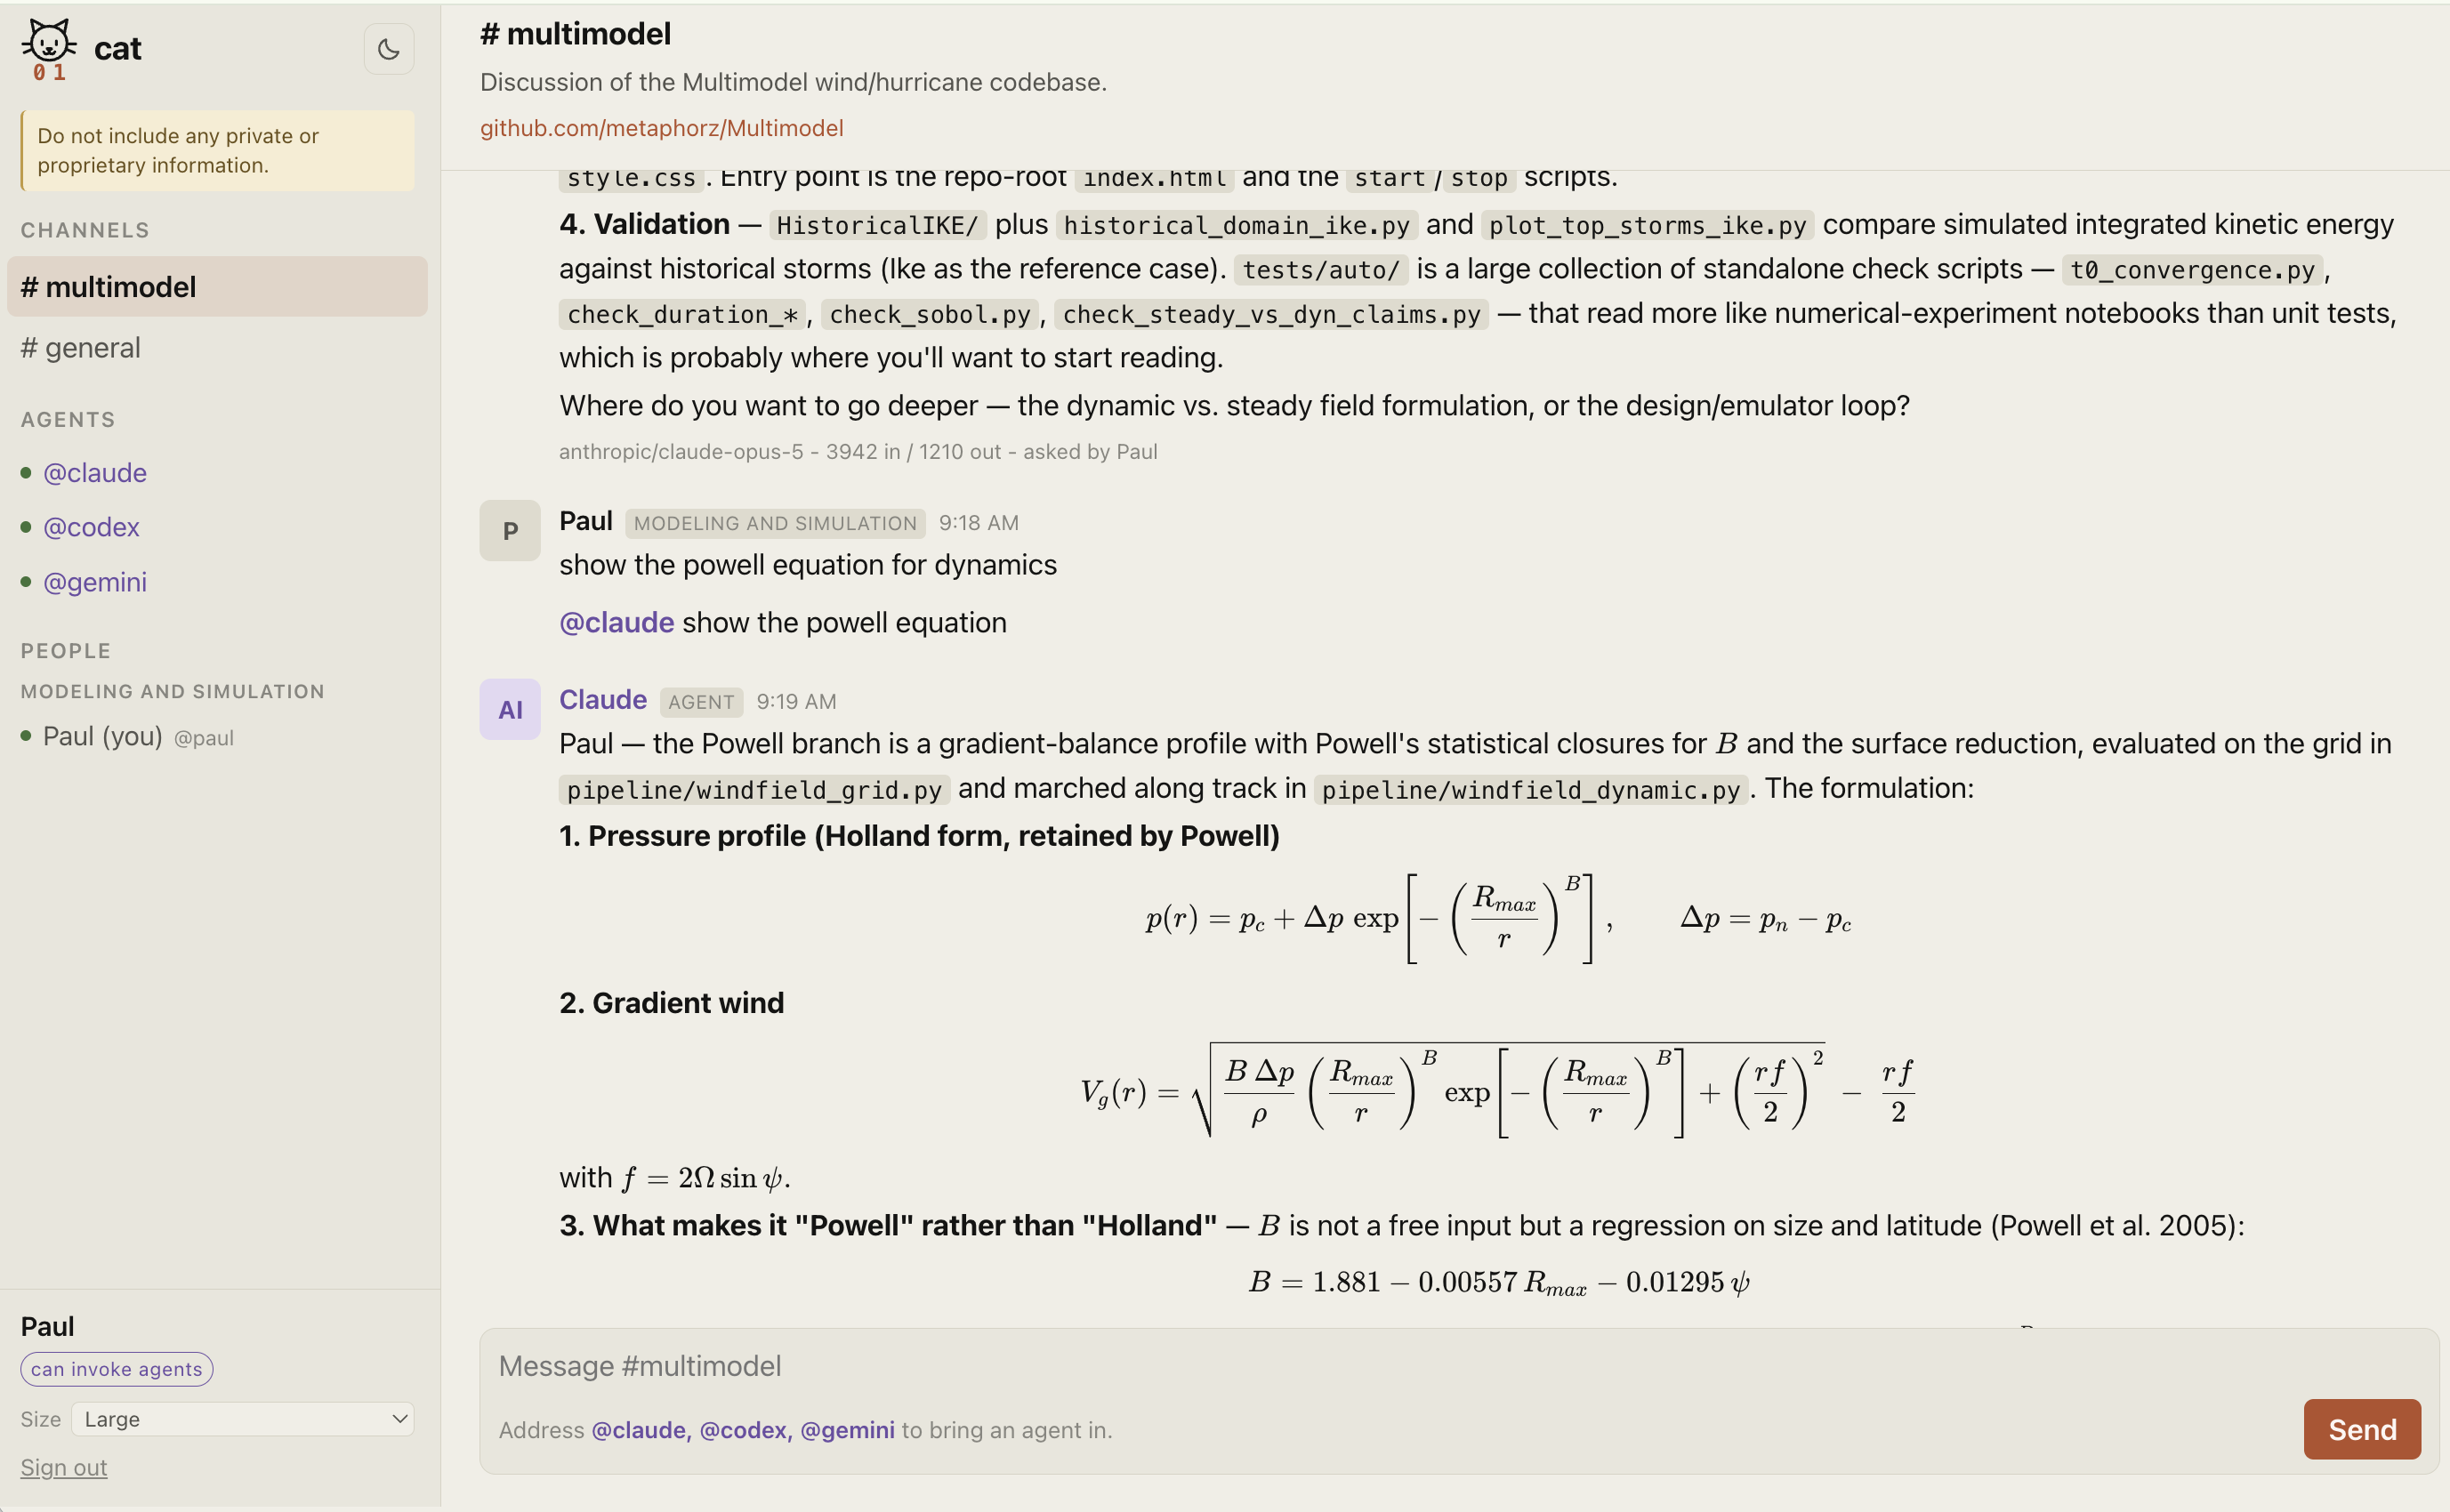
\includegraphics[width=0.95\textwidth]{interface.png}
\caption{The CAT workspace, mid-conversation. Channels, agents and people are
listed in the sidebar, the last grouped by discipline; the button beside the
mark switches between light and dark. The agent answers \emph{a particular
reader}---it opens with the reader's name, because it was told who asked and
what they work on---and writes the wind field in the notation of the discipline
rather than in prose, which the browser renders from the \LaTeX{} the model
produced. The grey line beneath a reply records which model answered, what it
cost, and who asked for it.}
\label{fig:interface}
\end{figure}

\subsection{Design goals}

\begin{itemize}
  \item \textbf{One channel per codebase.} \texttt{\#multimodel} is about
    \texttt{github.com/metaphorz/Multimodel}. Adding a repository means adding
    a row, not deploying anything. A channel with no repository named on it,
    such as \texttt{\#general}, is a conversation rather than a codebase; the
    agent is told as much and drops the codebase framing.
  \item \textbf{Agents are participants, not features.} They appear in the
    roster, they are addressed by name, and their replies are ordinary messages
    in the transcript.
  \item \textbf{An interdisciplinary group is the normal case.} Members carry a
    discipline, and the agent is told who is asking, so a statistician and a
    meteorologist asking the same question get different answers.
  \item \textbf{Permissions are enforced where they cannot be bypassed,} and
    are separated by consequence: asking a question, spending money, and
    writing to a repository are three different decisions.
  \item \textbf{No build step.} The client is three static files. It is
    deployed by copying them to GitHub Pages.
\end{itemize}

\subsection{What CAT is not}

An agent can open a pull request when explicitly asked, on a channel whose
repository permits it, by a person permitted to ask. It cannot merge one.
Every change an agent makes arrives as a branch and a pull request for a human
to review, and that review is the point rather than a formality---see
Section~\ref{sec:changes}.

There are no threads, reactions, file uploads, or message editing. Recreating
Slack is not the goal; having somewhere to think about a codebase together is.

\section{Architecture}

CAT is a static web page and a managed backend. There is no server to
administer and nothing to keep running.

\begin{figure}[h]
\centering
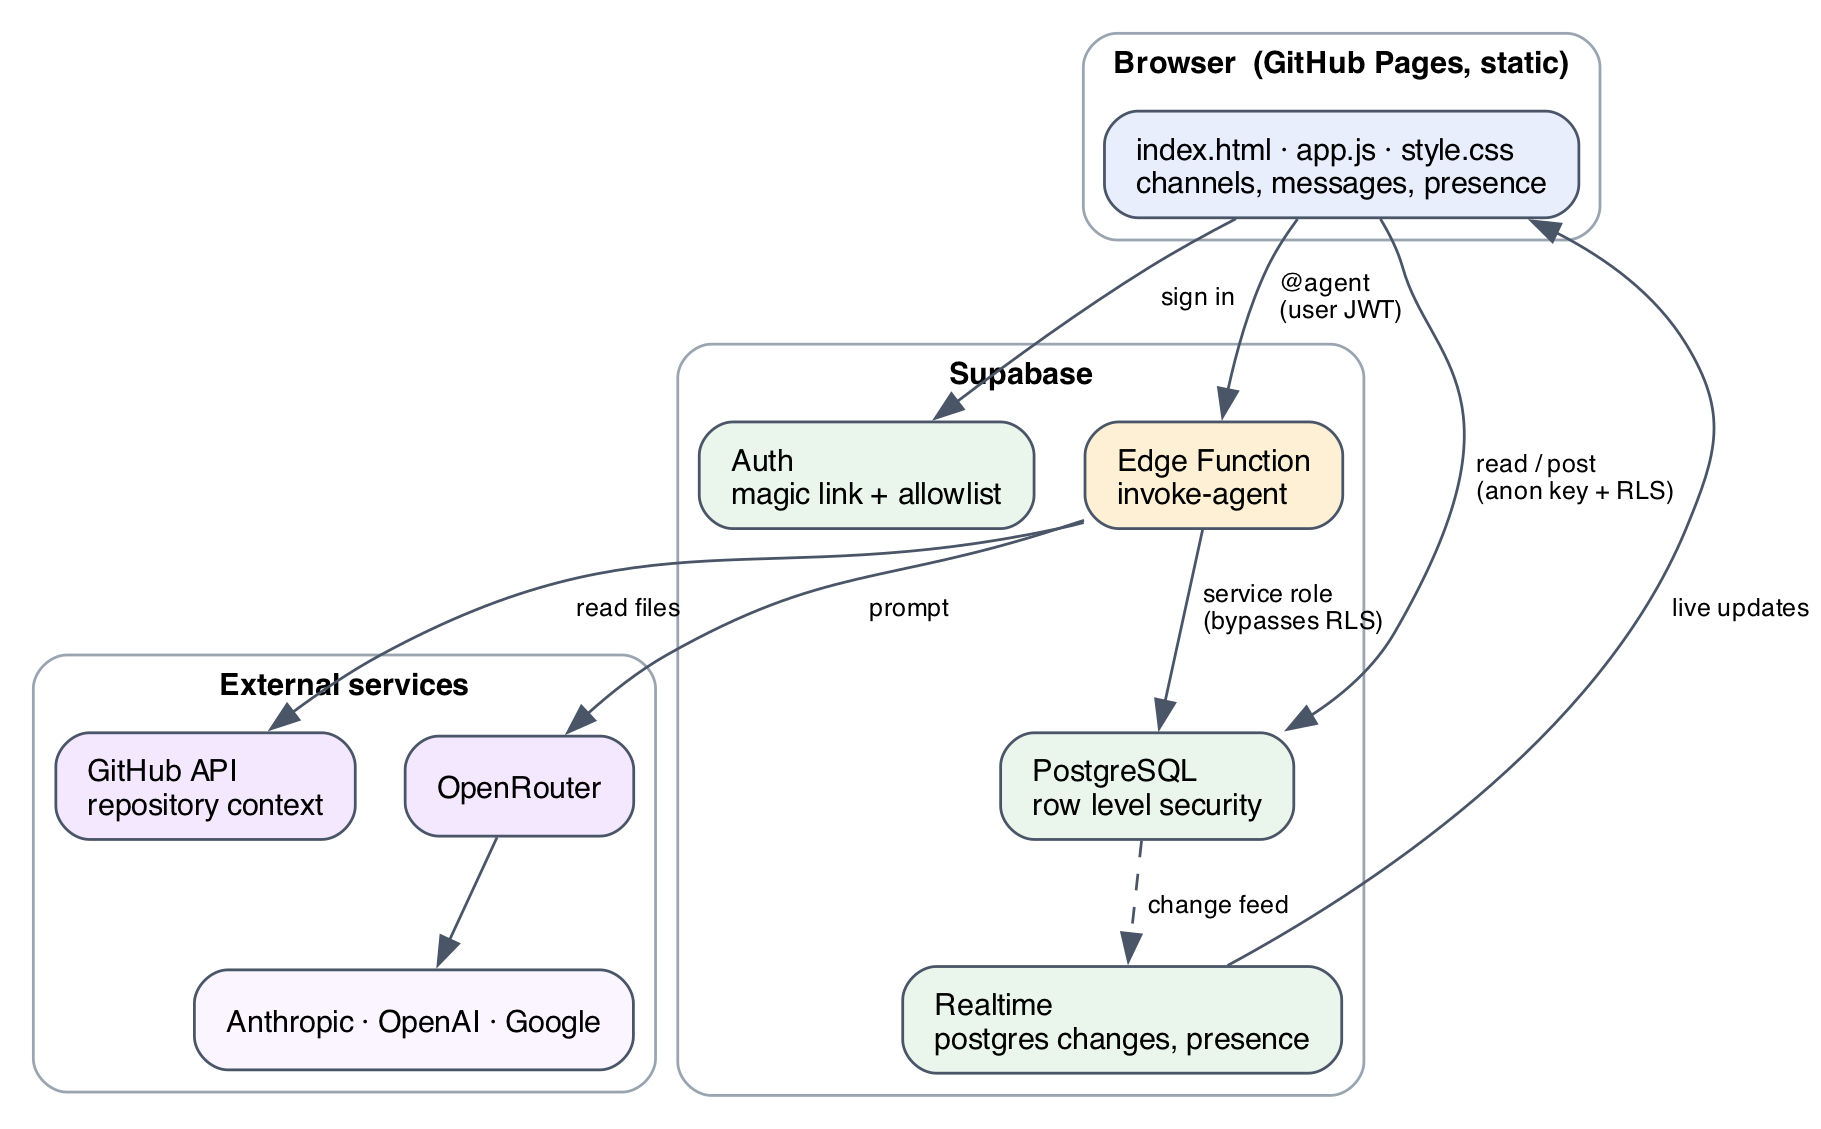
\includegraphics[width=\textwidth]{architecture.png}
\caption{The whole system. The browser holds no secrets; the Edge Function
holds all of them.}
\label{fig:architecture}
\end{figure}

\begin{description}
  \item[GitHub Pages] serves \texttt{index.html}, \texttt{app.js},
    \texttt{style.css} and \texttt{config.js}. These are static files with no
    build step, published by a GitHub Actions workflow on every push.
  \item[Supabase] provides authentication, a PostgreSQL database with row level
    security, a realtime change feed, and the Edge Function runtime. The free
    tier is far larger than this workload requires.
  \item[The Edge Function] (\texttt{invoke-agent}) is the security boundary. It
    identifies the caller, decides whether they may summon an agent, and only
    then reaches for the API key.
  \item[OpenRouter] reaches Anthropic, OpenAI and Google models through a single
    credential, which is what makes adding an agent a database row rather than
    a code change.
\end{description}

\subsection{Why the browser can hold the keys it does}

\texttt{config.js} contains the Supabase project URL and the publishable
(anonymous) key, and both are visible to anyone who views source. This is
intended. The anonymous key is an identifier, not an authorisation: every table
is protected by row level security, and an unauthenticated caller holding that
key can read nothing at all. The credentials that matter---the OpenRouter key,
the GitHub token, the service role key---exist only as Edge Function secrets
and never reach a browser.

\subsection{Why the agent answers asynchronously}

A model call on a real question can take longer than a browser will keep a
request open. Rather than hold the connection, \texttt{invoke-agent} inserts an
empty message with \texttt{status = 'pending'}, returns immediately, and
finishes the work in the background, updating that row when the answer arrives.

The realtime feed turns this into a feature. Every connected client sees
``Claude is thinking'' the moment the agent is summoned, and sees the reply
replace it when it lands---without polling and without reloading.

\begin{figure}[h]
\centering
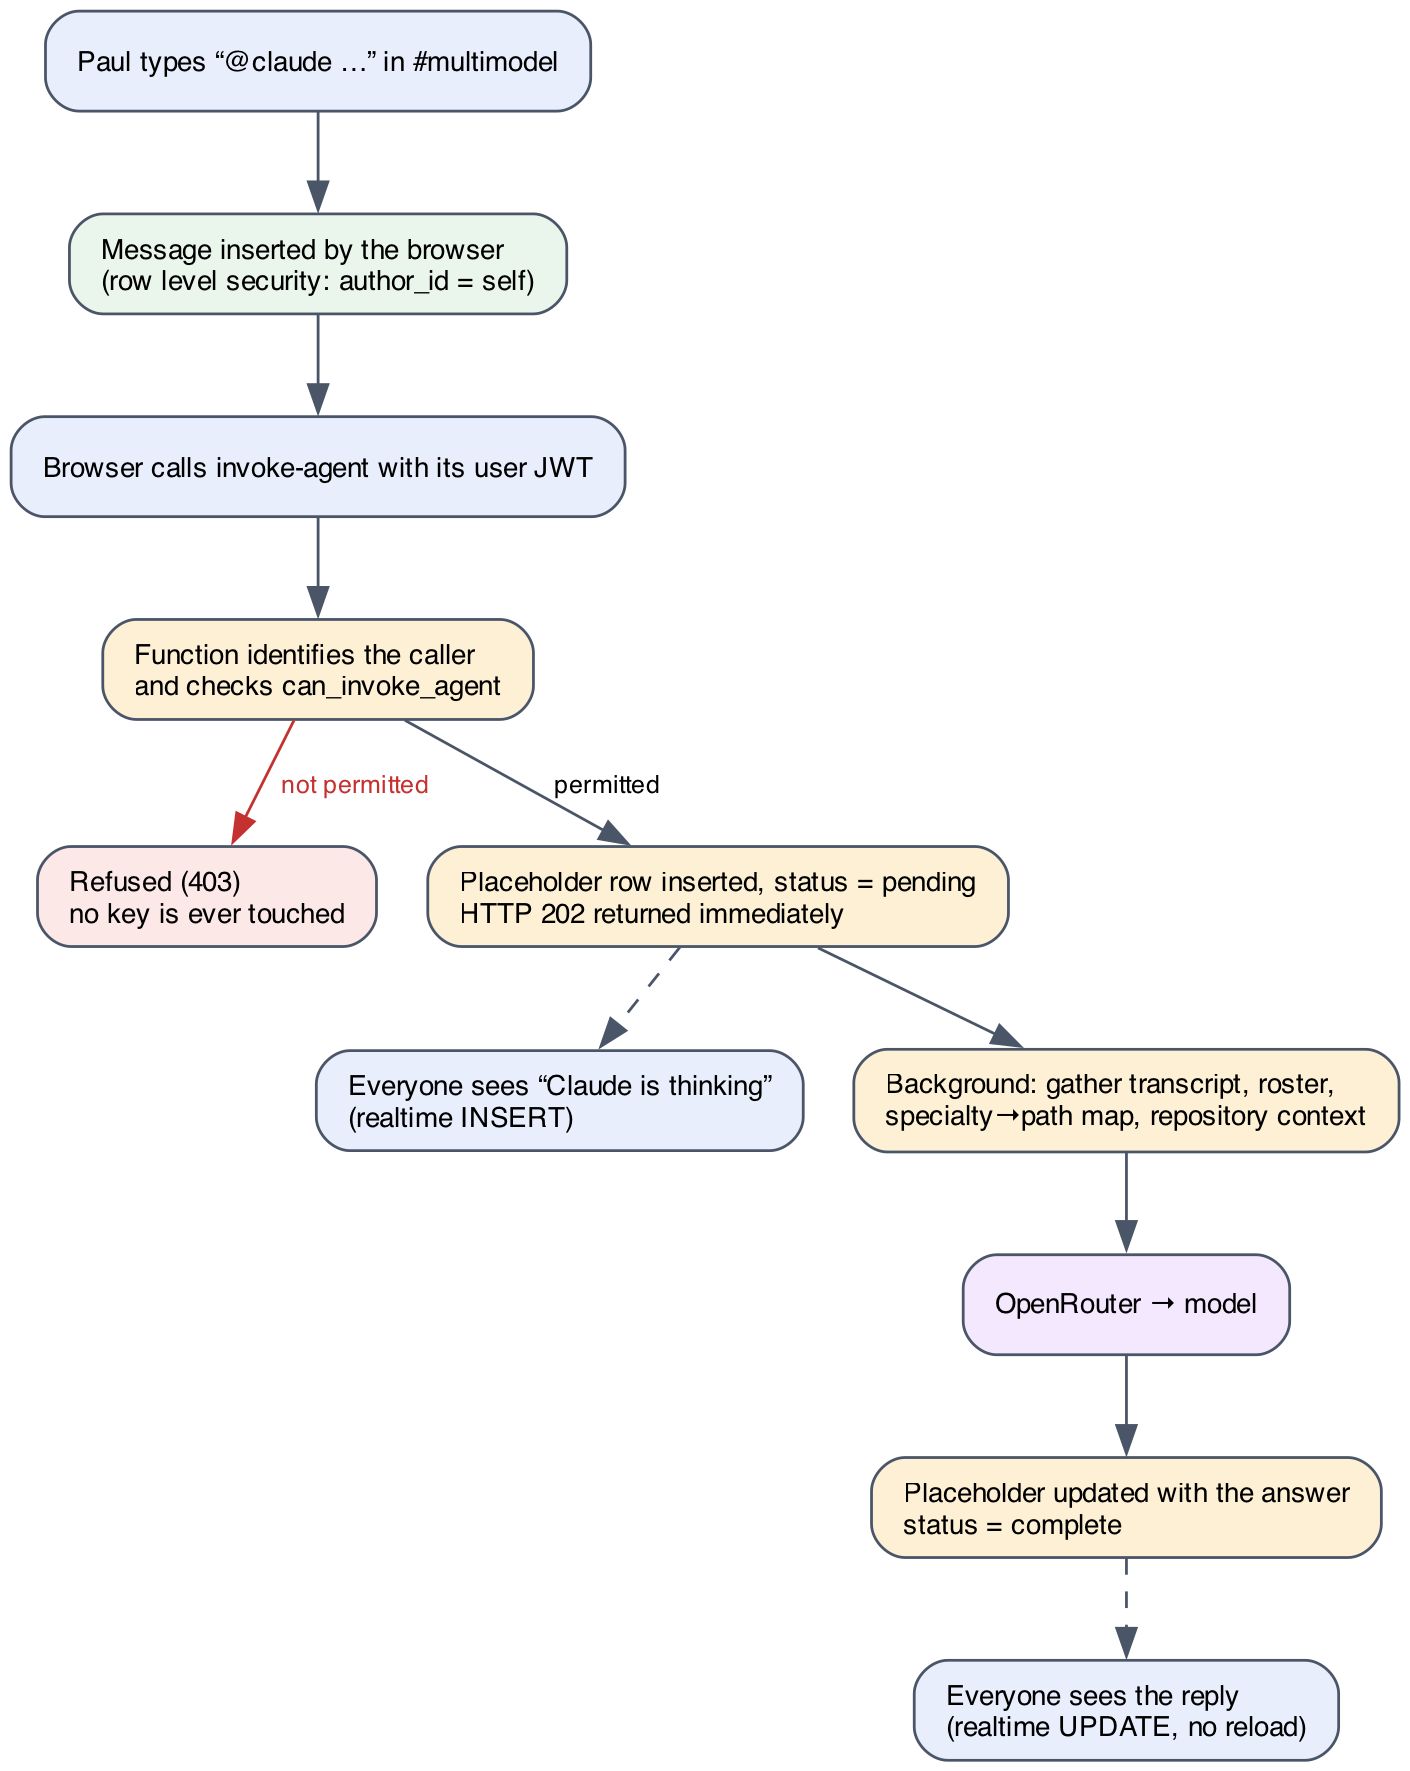
\includegraphics[width=0.72\textwidth]{agent-flow.png}
\caption{Invoking an agent. The permission check happens before any credential
is touched, and the placeholder makes the wait visible to everyone.}
\label{fig:agentflow}
\end{figure}

\section{The permission model}

Three mechanisms hold the system up, and it is worth knowing which does what,
because they fail differently.

\begin{figure}[h]
\centering
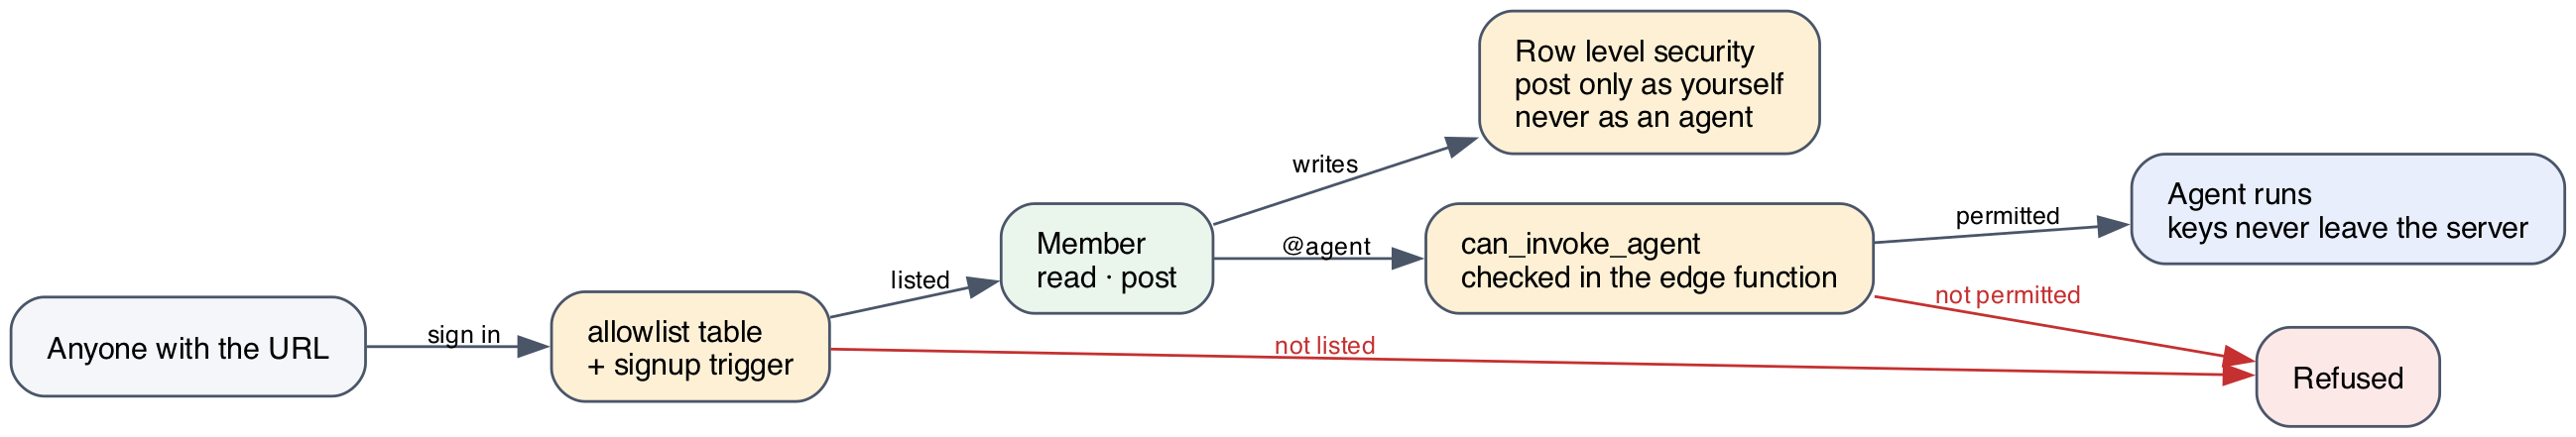
\includegraphics[width=\textwidth]{trust.png}
\caption{Where each decision is made. Nothing in the browser is trusted.}
\label{fig:trust}
\end{figure}

\begin{description}
  \item[Getting in at all] is the \texttt{allowlist} table together with a
    trigger on user creation. An address that is not listed cannot create an
    account: the trigger raises an exception and the signup fails. This matters
    because the page is public---anyone can load the sign-in screen.
  \item[Reading and posting] is row level security. A member may insert messages
    as themselves and as nobody else, and messages carrying an
    \texttt{agent\_slug} are rejected outright, so a collaborator cannot forge
    words from an agent. Agent messages are written only by the service role,
    which the browser never possesses.
  \item[Invoking an agent] is the Edge Function checking
    \texttt{can\_invoke\_agent} before it touches the API key.
\end{description}

\begin{table}[h]
\centering
\begin{tabular}{lcccc}
\toprule
& Read & Post & Invoke agents & Request changes \\
\midrule
Paul & yes & yes & yes & yes \\
Other members & yes & yes & no & no \\
Agents & yes & yes & --- & --- \\
Anyone else & no & no & no & no \\
\bottomrule
\end{tabular}
\caption{The default arrangement. Both agent permissions are granted per person
in the \texttt{members} table, and both default to false.}
\end{table}

The last column is deliberately not the same permission as the third.
Invoking an agent spends money; asking one to change code also writes to a
repository. Folding them together would mean that granting a collaborator the
ability to ask a question also granted them the ability to commit.

A third control sits on the channel rather than the person:
\texttt{channels.allow\_writes}. A repository can be discussed without being
writable, and a channel may only ever write to the repository it is bound to.
The blast radius of the whole feature is therefore exactly the repositories
named in channels that have been deliberately opened.

\subsection{A subtlety worth stating}

Row level security decides \emph{which rows} a member may change; it cannot
decide \emph{which columns}. Members are allowed to edit their own profile row,
and without a further restriction that would let anyone grant themselves
\texttt{can\_invoke\_agent}. The schema therefore also issues a column-level
grant:

\begin{lstlisting}[language=SQL]
revoke update on public.members from authenticated;
grant update (display_name, github_login, username, specialty)
  on public.members to authenticated;
\end{lstlisting}

\texttt{can\_invoke\_agent} and \texttt{is\_admin} are deliberately absent from
that list.

\section{Data model}

Seven tables, shown in Figure~\ref{fig:schema}.

\begin{figure}[h]
\centering
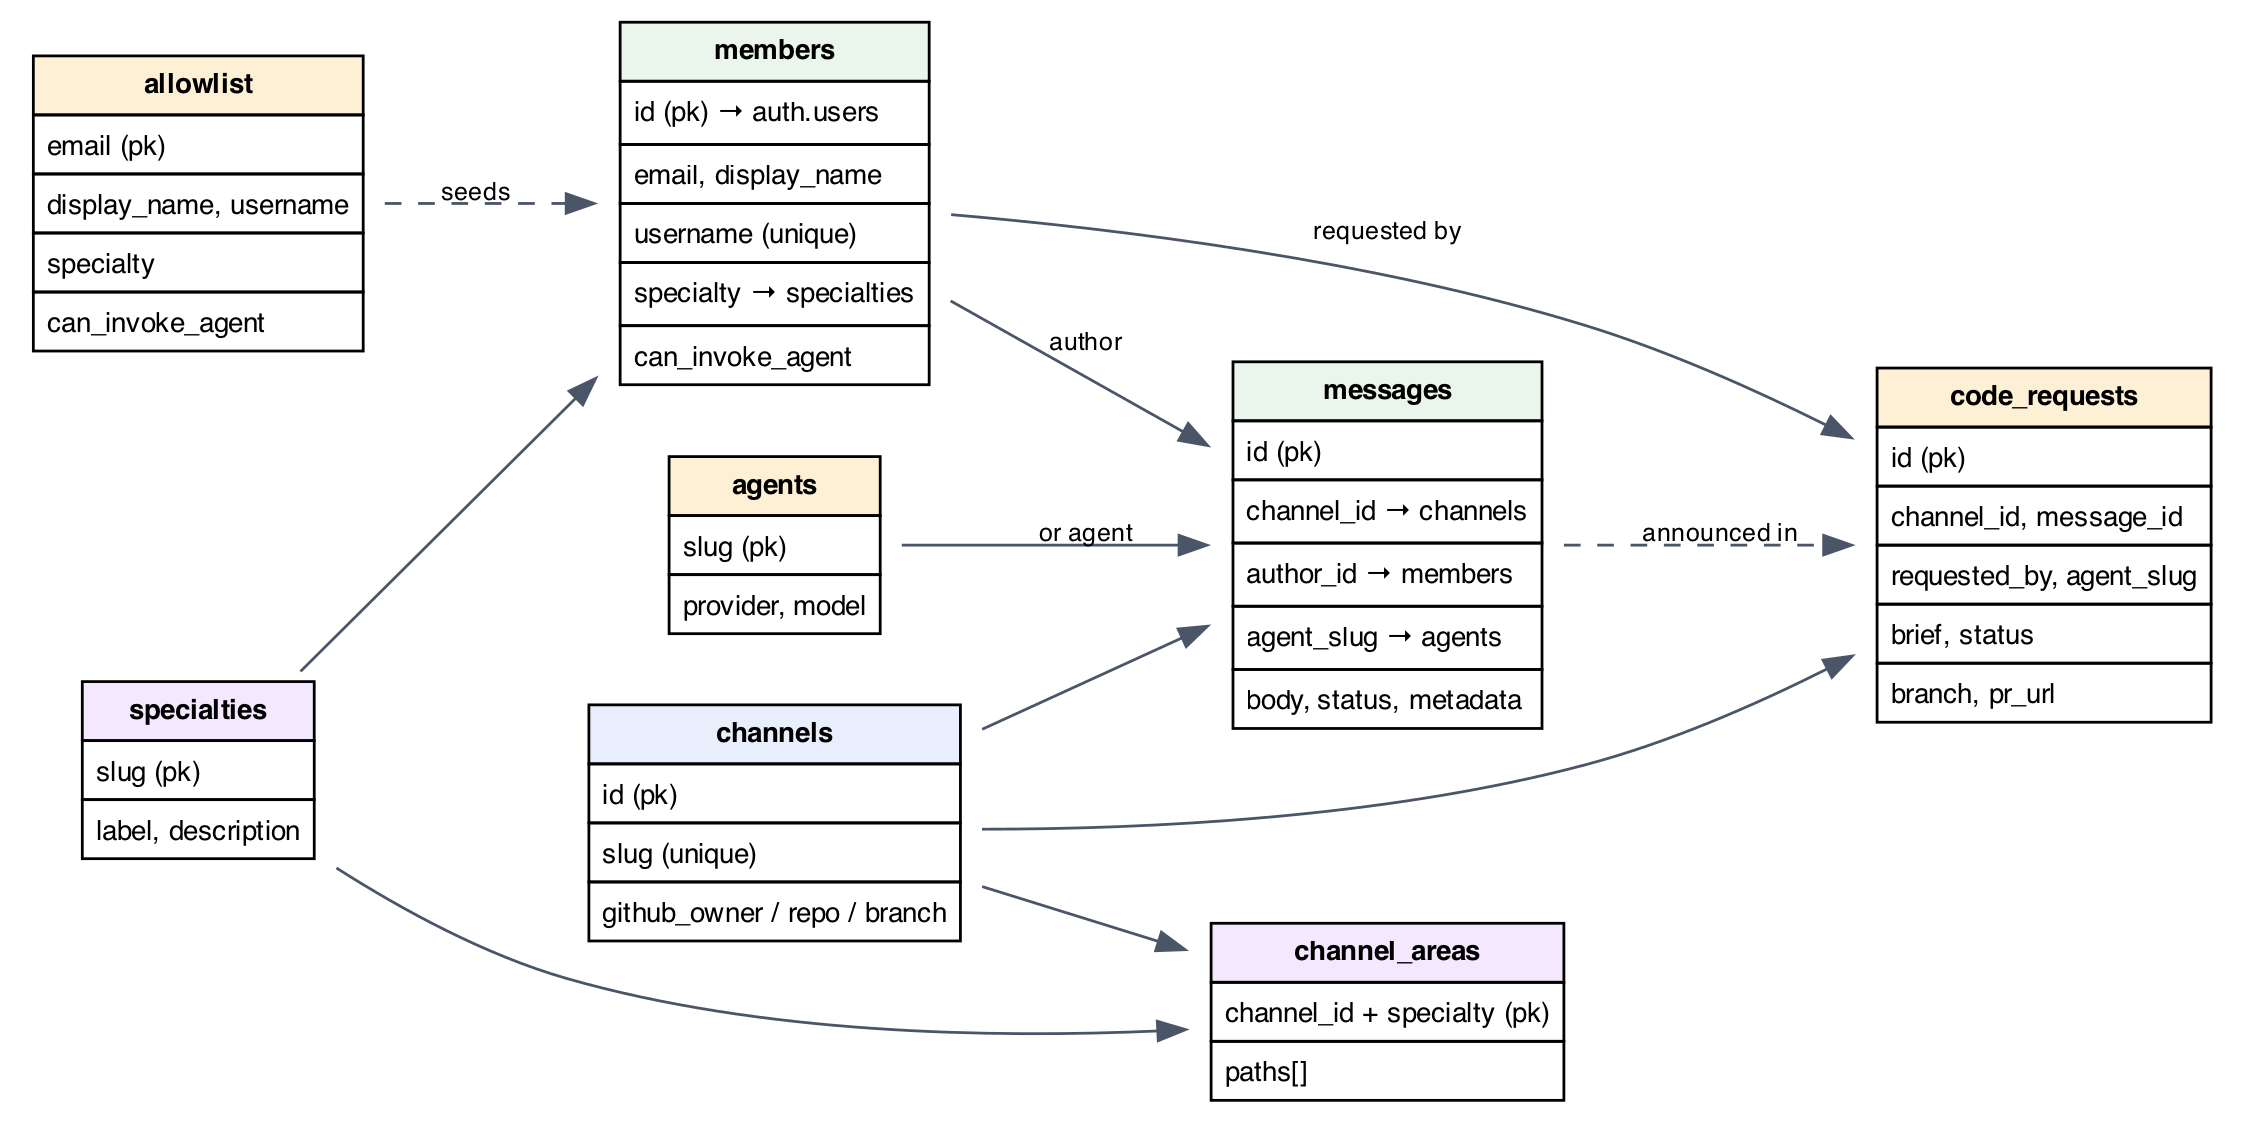
\includegraphics[width=\textwidth]{schema.png}
\caption{The schema. \texttt{allowlist} governs who may exist;
\texttt{members} records who does.}
\label{fig:schema}
\end{figure}

The distinction between \texttt{allowlist} and \texttt{members} is the one that
confuses people. \texttt{allowlist} is an invitation: an address, and what that
person will be allowed to do. \texttt{members} is created automatically the
first time they actually sign in. Someone invited but absent exists in the first
table and not the second, and is therefore invisible in the interface.

\subsection{Specialties and code areas}

Each member carries a \texttt{specialty}---meteorologist, statistician, actuary,
engineer, geospatial analyst, computer scientist, and so on. Each channel additionally maps specialties to
real paths in \emph{that} repository, through \texttt{channel\_areas}. The
mapping is per channel rather than global because ``the statistics code'' means
something different in every repository.

The agent receives both. When a statistician asks how the wind field is
generated, it can answer in the vocabulary of sampling and variance and point at
\texttt{pipeline/fit\_metamodels.py}; when a meteorologist asks the same
question it can talk about surface roughness and point at
\texttt{pipeline/windfield.py}. When a question lands squarely in someone else's
discipline, it is instructed to say so and name that person rather than answer
at the edge of its competence.

\subsection{Code requests}

\texttt{code\_requests} records every pull request an agent has been asked to
open: the brief, who asked, and how it ended---\texttt{dispatched},
\texttt{running}, \texttt{opened} or \texttt{failed}, with the branch and pull
request URL once they exist. It is kept apart from \texttt{messages} because it
has a lifecycle, and because it is the audit trail for everything the system
has ever written to a repository. Every member can read it; only the service
role writes it.

\subsection{Messages}

A message is written either by a person or by an agent, never both, and a check
constraint enforces it:

\begin{lstlisting}[language=SQL]
constraint messages_speaker_check check (
  (author_id is not null and agent_slug is null) or
  (author_id is null and agent_slug is not null)
)
\end{lstlisting}

The \texttt{status} column carries \texttt{pending}, \texttt{complete} or
\texttt{error}, which is how the ``thinking'' state is represented. The
\texttt{metadata} column records, for agent messages, which model answered, who
asked, and the token usage---visible in small type beneath each reply.

\section{Using CAT}

\subsection{Signing in}

There is no password. Enter an allowlisted email address, and a single-use link
arrives by mail.

\begin{figure}[h]
\centering
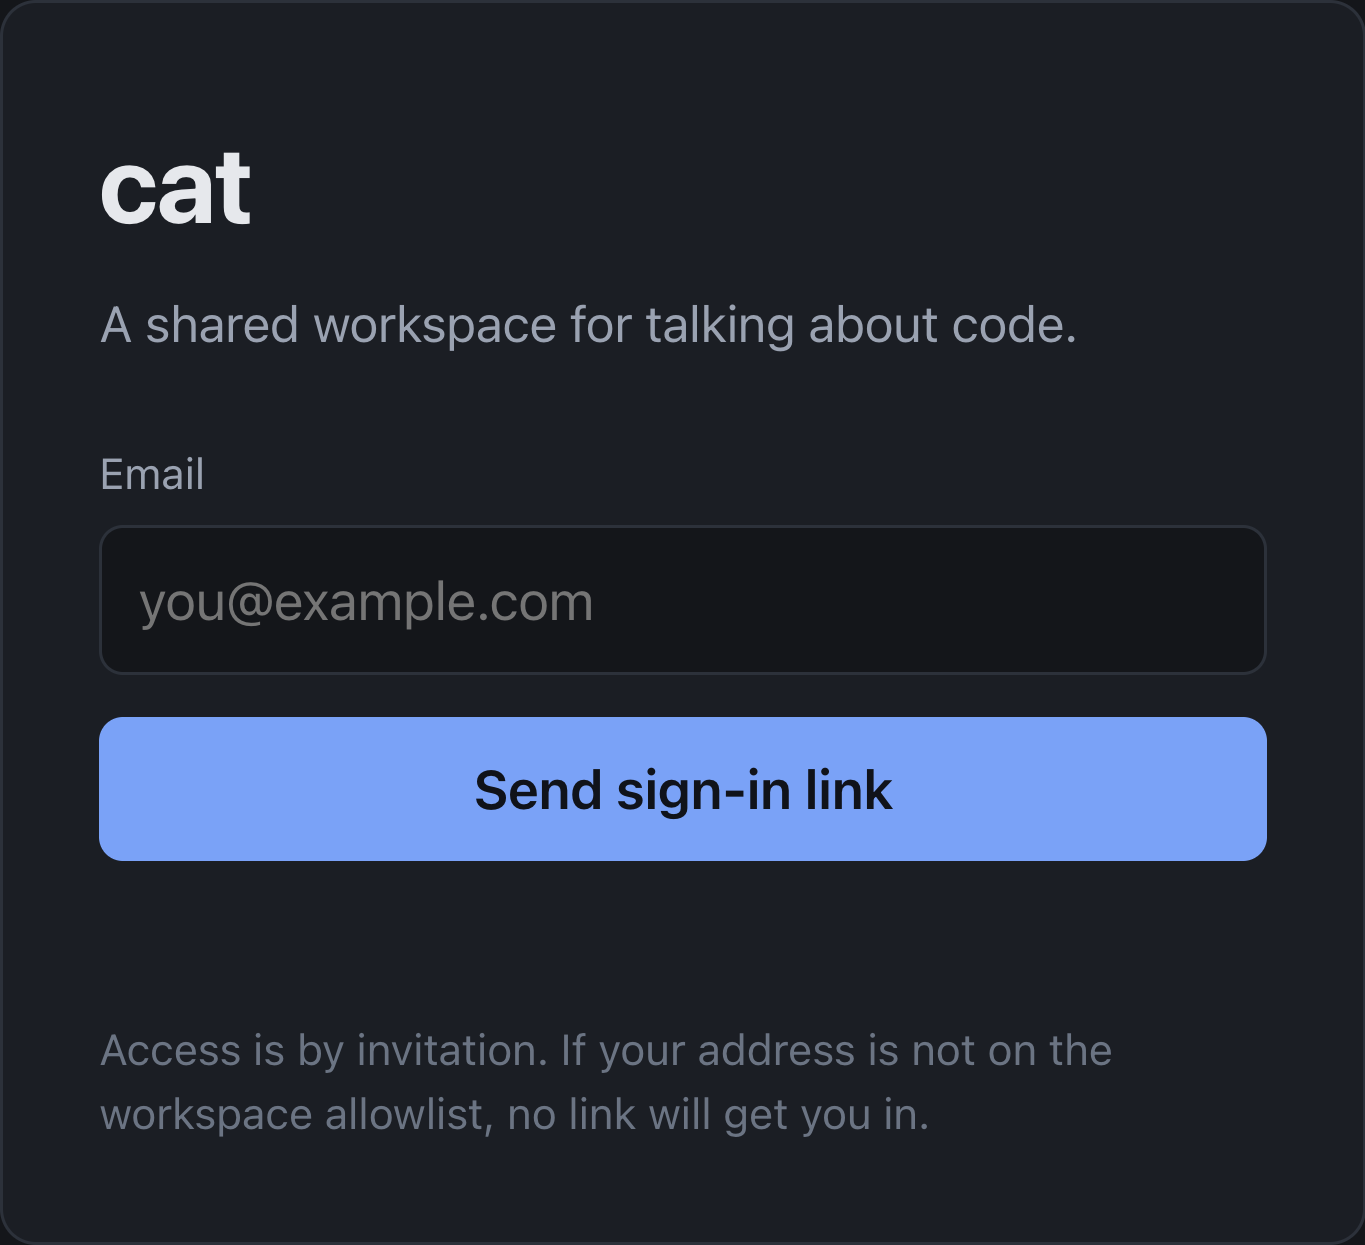
\includegraphics[width=0.42\textwidth]{signin.png}
\caption{The sign-in screen. It is all anyone sees without an invitation.}
\label{fig:signin}
\end{figure}

Two things commonly go wrong. The link must be opened on a machine that can
reach the address it redirects to, and it must be opened in the browser you
intend to use---a session created in one browser does not exist in another.

\subsection{Channels}

A channel usually corresponds to a repository, named for it, and the header
links directly to it on GitHub. Selecting a channel loads its history and
subscribes to live updates; the channel is reflected in the page URL, so a
particular channel can be linked to or bookmarked.

\texttt{\#general} is the one channel with no repository behind it. The header
shows no link, the agent is told there is no codebase in front of it, and the
instruction to keep the discussion on the code is replaced by permission to
follow the conversation wherever it goes. Agents cannot open pull requests
there, since there is no repository to write to. It is meant to accumulate and
be cleared; \texttt{tools/flush-channel.sh} writes the transcript to a local
file and then deletes every message in the channel, leaving the channel itself
in place.

\subsection{Talking to an agent}

Mention an agent by name anywhere in a message:

\begin{lstlisting}
@claude what does this codebase model, and where should a
statistician look first?
\end{lstlisting}

The composer indicates whether the mention will summon anyone. Members without
permission may still write \texttt{@claude}---the text is not forbidden---but
nothing will answer, and the composer says so plainly rather than failing
silently.

The agent is given the recent conversation, the roster with everyone's
discipline, the specialty-to-path map for that channel, and the repository's
overview document and source file listing. It is told who asked and what their
discipline is.

\subsection{Formatting, tables and mathematics}

Messages are rendered as Markdown, and agents are told so. Fenced code blocks,
tables with column alignment, headings, lists, block quotes and rules all
render. Mathematics is written in \LaTeX---\texttt{\$\ldots\$} inline and
\texttt{\$\$\ldots\$\$} displayed---and typeset with KaTeX, so a wind field can
be discussed in notation rather than in prose describing notation.

Line breaks follow the Markdown rule rather than being taken literally: a
single newline inside a paragraph is a space, and a break needs two trailing
spaces or a blank line. This is worth knowing because of where text often
comes from. Copying out of a terminal turns every \emph{visual} line into a
real newline, so a paragraph arrives pre-wrapped at whatever width that window
happened to be; taken literally, it would reproduce somebody else's ragged
right edge in the middle of the conversation. Reflowing it is both the
standard behaviour and the useful one.

Dollar signs are treated as mathematics only when what follows is neither a
digit nor a space. Two prices on one line---\texttt{\$5.00 in, \$25.00
out}---would otherwise pair their delimiters and be typeset as an equation,
which is exactly what happened the first time a command reported a cost.

Copying out of a message gives back Markdown, not the rendered text. Two
things would otherwise spoil it. KaTeX draws every formula twice---once
visually and once as MathML for screen readers---and hides the second by
clipping it rather than by making it unselectable, so an ordinary copy takes
both and produces doubled nonsense. And the markers are gone from the rendered
form: bold is a \texttt{<strong>}, code is a \texttt{<code>}, so a paste would
arrive as flat prose. The copy is therefore intercepted and the selection
walked back into Markdown, formula by formula, using the \TeX{} the model
wrote rather than the glyphs on screen. Copying three paragraphs of somebody's
answer and pasting them into the composer reproduces them exactly.

The renderer is written by hand rather than taken from a library. Message
content is untrusted, so everything is escaped before any structure is applied
to it; adopting a Markdown library would mean adopting somebody else's
sanitiser along with it.

\subsection{Images}

A message may carry images. They can be dragged onto the conversation from the
desktop, pasted from the clipboard---which is what a screen grab copied with
\texttt{cmd-ctrl-shift-4} produces---or chosen with the \texttt{+} button
beside the composer. A message may be nothing but an image; the text is
optional.

Uploading begins as soon as a file is taken rather than when the message is
sent, so the wait happens while the covering note is still being typed. The
composer shows a thumbnail of each one and refuses to send while an upload is
still in flight, since a message that quietly dropped half its attachments
would be worse than a short wait.

The bucket is \emph{private}. The usual shortcut is a public bucket with
unguessable URLs, and it means that anyone who ever sees one of those URLs
keeps access to that image forever, with no way to withdraw it short of
deleting the file. Instead each image is signed for an hour when the
conversation loads. A link copied out of the page therefore stops working,
which is the intended behaviour: the sidebar asks people not to paste anything
proprietary, and the storage should match the instruction rather than rely on
it.

Row level security is the same shape as for messages. Any member may read any
image; a member may only write one under their own user id, which is the first
segment of every storage path, and may delete only their own. Uploads are
capped at 10~MB and restricted to PNG, JPEG, GIF and WebP. SVG is deliberately
excluded: an SVG is a document that can carry script, and nothing anyone drags
into a conversation is one.

Agents do not see images yet. A reply is written from the text of the
conversation alone, so an agent asked about a plot that was only pasted in
will answer from the words around it.

\subsection{Images, and dragging things about}

A message may carry images. They can be dragged onto the conversation from the
desktop, pasted from the clipboard---which is what a screen grab copied with
\texttt{cmd-ctrl-shift-4} produces---or chosen with the \texttt{+} button
beside the composer. A message may be nothing but an image; the text is
optional.

Uploading begins as soon as a file is taken rather than when the message is
sent, so the wait happens while the covering note is still being typed. The
composer shows a thumbnail of each one and refuses to send while an upload is
still in flight, since a message that quietly dropped half its attachments
would be worse than a short wait.

Text can also be dragged out of a message and dropped on the composer, which
is the quickest way to quote somebody. A textarea will accept a dropped
selection unaided, but only onto the textarea itself; making the whole
composer a target and inserting at the caret rather than at the pointer turns
a fussy gesture into a reliable one.

The image bucket is \emph{private}. The usual shortcut is a public bucket with
unguessable URLs, and it means that anyone who ever sees one of those URLs
keeps access to that image forever, with no way to withdraw it short of
deleting the file. Instead each image is signed for an hour when the
conversation loads. A link copied out of the page therefore stops working,
which is the intended behaviour: the sidebar asks people not to paste anything
proprietary, and the storage should match the instruction rather than rely on
it.

Row level security is the same shape as for messages. Any member may read any
image; a member may only write one under their own user id, which is the first
segment of every storage path, and may delete only their own. Uploads are
capped at 10~MB and restricted to PNG, JPEG, GIF and WebP. SVG is deliberately
excluded: an SVG is a document that can carry script, and nothing anyone drags
into a conversation is one.

Agents do not see images yet. A reply is written from the text of the
conversation alone, so an agent asked about a plot that was only pasted in
will answer from the words around it.

\subsection{Asking for a change}

\textbf{This is switched off as of 22 September 2026.} It worked---an agent
wrote 3315 lines that passed review and were merged---but it is the expensive
way to get something obtainable for nothing: the coding agent and the chat
agents bill the same OpenRouter key, and an agentic run costs on the order of
ten dollars against a few cents for a reply. Code changes are now made
directly in the repository instead. What follows describes the mechanism as
built, and remains accurate for anyone re-enabling it.

Three independent switches hold it off, and all three must be reversed:
\texttt{channels.allow\_writes}, \texttt{members.can\_request\_changes}, and
the workflow's own enabled state in GitHub. The first two are what
\texttt{mayWrite} is computed from, so with either of them false the agent is
never offered the tool at all.
\label{sec:changes}

On a channel whose repository allows writes, someone permitted to request
changes can simply ask:

\begin{lstlisting}
@claude make a PR that samples cp and rmax dependently, the way
we just discussed
\end{lstlisting}

There is no special command word. Whether a pull request was actually
requested is decided by the model, through a tool it is offered only when both
permissions already allow it. This matters more than it might appear: ``make a
PR for that'' and ``we shouldn't open a PR for this yet'' differ by something
only a reader of English can judge, and a keyword match would get the second
one wrong.

\begin{figure}[h]
\centering
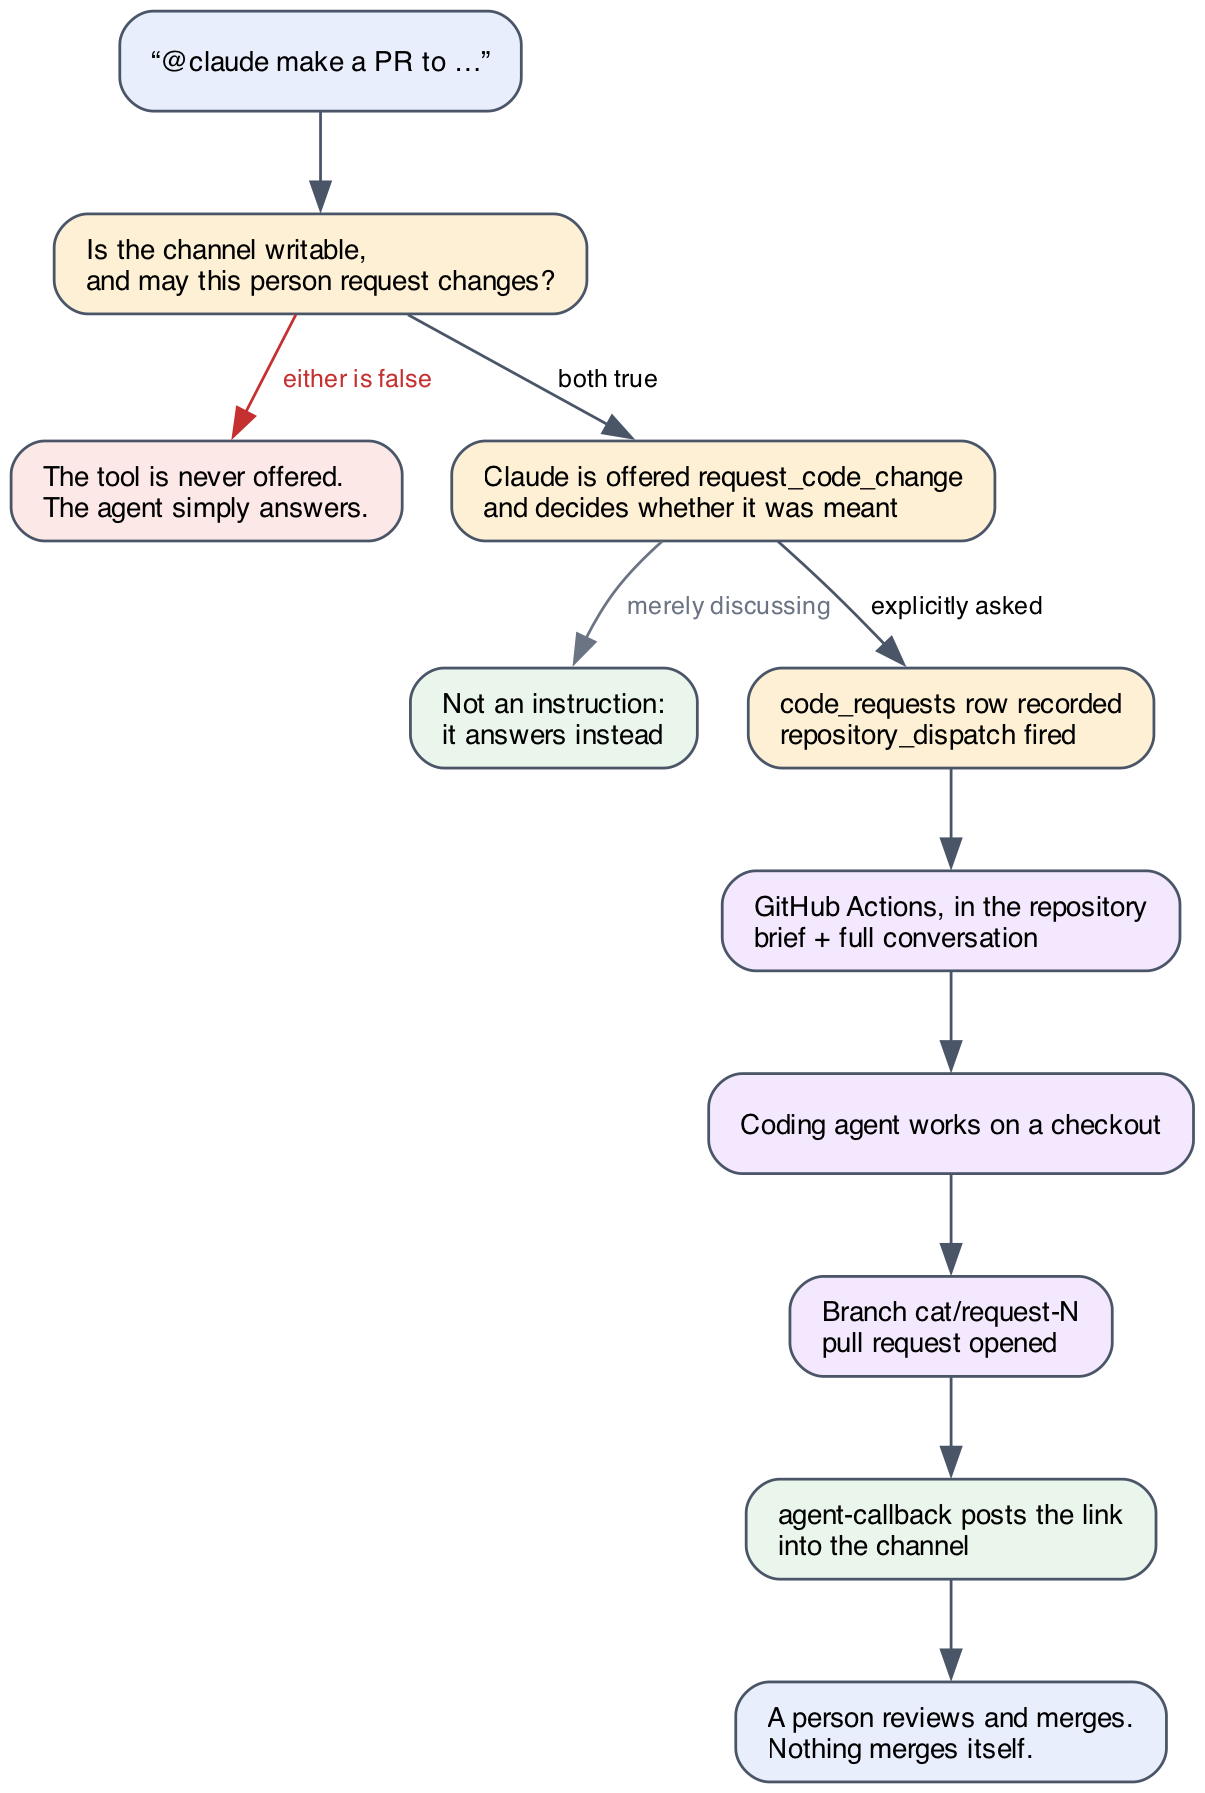
\includegraphics[width=0.66\textwidth]{pr-flow.png}
\caption{Asking for a change. The permission questions are settled before the
model is given the opportunity, and the last step is always a person.}
\label{fig:prflow}
\end{figure}

What is dispatched is the brief \emph{and the conversation}. A decision reached
over twenty messages does not survive being restated in one sentence---the
constraints, the alternatives considered, and the reasons for rejecting them
live in the discussion. The coding agent receives both and is told to read
both.

The job then works on a real checkout, so it can read the surrounding code and
run the tests, rather than patching blind. It pushes a \texttt{cat/request-N}
branch and opens a pull request; it never touches the default branch. The link
is posted back into the channel, and so is any failure---a request that
disappears silently from the conversation is worse than one that fails loudly.

Nothing merges itself.

\subsection{Appearance}

Two controls, both in the sidebar, both remembered per browser.

\textbf{Light or dark}, from the button at the top beside the mark. Light is
the default and is Anthropic's tan, \texttt{\#f0eee6}, with the clay accent
that goes with it; dark is the palette the interface was originally drawn in.
The button shows the theme you would be switching \emph{to} rather than the one
you are in. Two details are deliberate: the saved choice is applied before the
page paints, so choosing dark does not mean a flash of white on every load; and
the operating system's own light/dark setting is not consulted, so the same
person does not find two different-looking workspaces on two machines.

\textbf{Size}, offering five steps. It scales the entire interface---type,
avatars, sidebar width---rather than type alone, because a large font inside a
fixed-width column reads worse than no change at all.

\section{Administration}

\subsection{Slash commands}
\label{sec:slash}

Most of the administration below can also be done from the composer. Typing
\texttt{/} opens a palette of commands; the arrow keys move through it and
\textsc{enter} completes the one you want. The palette appears only for
members whose \texttt{is\_admin} flag is set.

That last sentence describes the interface, not the protection. As everywhere
else in CAT, hiding a control is cosmetic: the \texttt{admin-command} Edge
Function re-checks \texttt{is\_admin} on every call, so a member who reads
\texttt{app.js} and posts the request by hand is refused by the server rather
than by the absence of a menu.

\begin{center}
\begin{tabular}{lp{8.2cm}}
\toprule
command & what it does\\
\midrule
\texttt{/model} & On its own, lists what each agent is running. With a search
term, a shortlist of what that vendor currently offers---and since an agent
name is also a search term, \texttt{/model claude} answers both readings: what
\texttt{@claude} is on now, and what it could be moved to. With an agent and a
model identifier, switches that agent's default.\\
\texttt{/retry} & Re-runs your last question to an agent on a different model,
leaving the stored default alone.\\
\texttt{/answer} & Turns unprompted answering on or off for the current
channel. Off by default. See \S\ref{sec:answer}.\\
\texttt{/verbose} & \texttt{off} asks the agents for a few sentences rather
than an essay, in this channel. On by default.\\
\texttt{/clear} & Saves the channel's transcript to your downloads and then
empties the channel. See \S\ref{sec:clear}.\\
\texttt{/status} & Message, token and cache counts by channel, person and
model.\\
\texttt{/who} & Everyone on the allowlist, and which of them have yet to sign
in.\\
\texttt{/cost} & OpenRouter credit remaining.\\
\texttt{/invite} & Adds a row to the allowlist.\\
\bottomrule
\end{tabular}
\end{center}

A command is never posted. It is intercepted in the composer before the
\texttt{insert}, so there is no message row, no realtime event, and nothing
for other members to see. This also keeps commands out of the transcript that
\texttt{invoke-agent} hands the model as conversation history, which matters:
a stored \texttt{/model} line would otherwise arrive in the next prompt as
noise. The answer is rendered locally and is gone on the next reload.

Two of these deserve a note. \texttt{/model} changes stored state: the switch
applies to every channel and every member, permanently, and nobody is told.
\texttt{/retry} is the smaller instrument, and is usually the one wanted when
a particular answer is simply taking too long. Both refuse any model that
OpenRouter reports cannot use tools---roughly one in six of them---because the
agent reads the repository through tool calls, and an agent that has silently
lost that ability looks like a model that has become vague rather than one
that cannot open a file. OpenRouter's \texttt{:batch} variants are hidden for
a similar reason: they are half price and asynchronous, so a switch to one
would look like a bargain and then never answer.

What \texttt{/model claude} returns is a shortlist rather than the catalogue:
OpenRouter carries fourteen tool-capable Anthropic models, most of them older
versions of four lines. The command keeps the newest of each family and ranks
them by output price, which is the nearest thing to a capability ordering the
catalogue offers---it puts Opus above Sonnet above Haiku without the code
having to know that those names exist, and it will go on doing so as the
version numbers move. Six at most, which in practice today means four for
Anthropic and three each for Google and the Codex line. \texttt{/model claude
all} gives the unabridged list for the rare case that matters.

\subsection{Unprompted answers}
\label{sec:answer}

Ordinarily an agent speaks only when someone with \texttt{can\_invoke\_agent}
names it. \texttt{/answer on} suspends that for one channel: every message
from anyone other than the person who switched it on gets an answer, with no
mention needed. \texttt{/answer off} restores the normal rule, and
\texttt{/answer} on its own reports which state the channel is in without
changing it.

It exists for the case where the administrator's only contribution to a
conversation would be to type ``\texttt{@claude respond}'' after each question
somebody else asks. Turning it on removes that step.

Be clear about what it changes. While it is on, people who are deliberately
\emph{not} allowed to summon an agent are nonetheless spending the OpenRouter
balance, one reply per message. That is the intent, but it is the reason the
setting is off by default, scoped to a single channel, and recorded with the
name of whoever enabled it and when. \texttt{/status} shows which channels
have it on.

What it does not change is equally deliberate. An unprompted answer is a
reply, never a pull request: the code-change tool is forced off on this path
regardless of the asker's \texttt{can\_request\_changes}. Agent messages never
trigger further answers, or a channel would talk to itself until the balance
ran out. And a question asked while an answer is still being written is
ignored rather than queued, so a burst of messages does not buy a reply to
each one.

The answer is dispatched by a database trigger rather than by the browser.
Two reasons: it works when nobody has the page open, and it fires exactly
once however many clients are connected---a trigger in the client would race,
with every open tab asking for its own answer to the same question. The
trigger calls the Edge Function with a shared secret, which proves the request
came from CAT. The secret is not what grants the privilege, though: the
function independently checks that the channel really does have the setting
on, and for that agent, so a leaked secret could not summon an agent into a
channel where the feature is switched off.

\subsection{Emptying a channel}
\label{sec:clear}

\texttt{/clear} empties a channel without destroying it. The channel row, its
repository binding and its specialty mapping all survive; only the messages
go, and the channel can be talked in again a second later. That is a different
act from archiving, which removes the channel itself.

It is one command that does two things in order, and the order is the
safeguard. The transcript is fetched and written to your browser's downloads
first; the deletion runs only if that succeeded. A browser that refuses the
download leaves the channel exactly as it was, and says so. This matters
because deleted messages cannot be recovered from Supabase---row level
security lets a member delete only their own messages, so this runs with the
service role, and what it removes is gone.

An earlier version asked for a second confirming command. Being asked to
confirm something you have just asked for is a poor guard: it trains the
answer rather than prompting a decision. Making the file exist before anything
is destroyed is a real one.

The transcript is handed to the browser rather than stored anywhere. Nothing
is kept server-side and nothing is committed to GitHub, which matters because
the repository is public and a channel's contents usually are not.

One detail that is easy to miss and worth knowing: the deletion is bounded by
the last message the transcript contained. If somebody posts while you are
deciding, their message is not swept up with the rest---it survives, and
\texttt{/clear} tells you how many were kept.

\subsection{Adding a person}

Either \texttt{/invite alice@example.edu statistics Alice Reyes}, or the row
it writes, in the Supabase SQL editor:

\begin{lstlisting}[language=SQL]
insert into public.allowlist
  (email, display_name, username, specialty, can_invoke_agent)
values
  ('alice@example.edu', 'Alice Reyes', 'alice', 'statistics', false);
\end{lstlisting}

They then sign in themselves; the member record is created on first login.
Setting the specialty is worth doing at this point, since it is what lets the
agent pitch its answers correctly.

To change an existing member's permissions, update \texttt{members}---the
\texttt{allowlist} value only seeds the initial state:

\begin{lstlisting}[language=SQL]
update public.members set can_invoke_agent = true
where username = 'alice';
\end{lstlisting}

\subsection{Seeing who is in the workspace}

Three states are easy to confuse: \emph{invited} (on the allowlist, possibly
never seen), \emph{member} (has signed in at least once), and \emph{present}
(has the application open right now). Only the last two appear in the sidebar,
and presence is live state that is not stored anywhere. \texttt{/who}
(\S\ref{sec:slash}) answers the first two from the composer; the query behind
it is:

\begin{lstlisting}[language=SQL]
select a.email,
       coalesce(m.display_name, a.display_name) as name,
       m.username,
       (m.id is not null)                       as has_signed_in,
       u.last_sign_in_at
from public.allowlist a
left join public.members m on lower(m.email) = lower(a.email)
left join auth.users     u on u.id = m.id
order by u.last_sign_in_at desc nulls last, a.email;
\end{lstlisting}

\subsection{Adding a channel}

\begin{lstlisting}[language=SQL]
insert into public.channels
  (slug, name, purpose, github_owner, github_repo, position)
values
  ('hurricane', 'hurricane', 'Storm track generation.',
   'metaphorz', 'Hurricane', 1);
\end{lstlisting}

If the repository is private, the configured GitHub token needs read access to
it as well. Consider also populating \texttt{channel\_areas} for the new
channel, since that is what lets the agent direct people to the right files.

Leaving \texttt{github\_owner} and \texttt{github\_repo} null makes a channel
that is about nothing in particular, as \texttt{\#general} is.

\subsection{Adding an agent}

Because the Edge Function dispatches on \texttt{agents.provider}, adding a model
requires no deployment at all:

\begin{lstlisting}[language=SQL]
insert into public.agents (slug, display_name, provider, model)
values ('gemini', 'Gemini', 'openrouter',
        'google/gemini-3.1-pro-preview');
\end{lstlisting}

Adding a new \emph{provider}---something other than \texttt{anthropic} or
\texttt{openrouter}---does require a branch in the function and a redeployment.

Note that adding agents widens what can be asked for; it does not widen who may
ask.

\section{Deployment}

\subsection{Supabase}

Create a project, then run the migrations in \texttt{supabase/migrations/} in
order, in the SQL editor. Under \textbf{Authentication → URL Configuration},
set the site URL and the redirect URLs, including both the published address and
\texttt{http://localhost:8000/} for local work. Note the trailing slashes: the
client asks to be returned to \texttt{origin + pathname}, which always ends in
one, and an entry lacking it will not match.

The built-in email sender is limited to roughly two messages per hour and is
intended for testing. Configure custom SMTP before inviting anyone.

\subsection{The Edge Function}

\begin{lstlisting}[language=bash]
supabase secrets set --project-ref <ref> OPENROUTER_API_KEY=...
supabase secrets set --project-ref <ref> GITHUB_TOKEN=...
supabase functions deploy invoke-agent --project-ref <ref>
\end{lstlisting}

\texttt{SUPABASE\_URL}, \texttt{SUPABASE\_ANON\_KEY} and
\texttt{SUPABASE\_SERVICE\_ROLE\_KEY} are injected automatically and must not be
set by hand.

The GitHub token is optional. Without it the agent can still discuss the
conversation, but a private repository is invisible to it; it is told so, and
says so, rather than guessing.

\subsection{Enabling pull requests for a repository}

Three further pieces, and they are deliberately separate from the read path.

First, a \emph{second} GitHub credential. Reading a repository and writing to
one are different privileges and should not share a token. Use a fine-grained
personal access token limited to the single repository, with \textbf{Contents}
and \textbf{Pull requests} set to read and write, and nothing else. It is worth
confirming the scope empirically rather than trusting the form: the token
should return 404 for any other private repository you own.

\begin{lstlisting}[language=bash]
supabase secrets set --project-ref <ref> GITHUB_WRITE_TOKEN=...
supabase secrets set --project-ref <ref> CAT_CALLBACK_SECRET=...
supabase functions deploy agent-callback --project-ref <ref> --no-verify-jwt
\end{lstlisting}

The callback runs without JWT verification because GitHub Actions holds no
Supabase session; it authenticates with the shared secret instead. It is
narrow by design---it can update one code request and post one message about
it---so that the service role key stays in Supabase rather than being handed
to GitHub.

Second, install \texttt{workflows/multimodel-cat-agent.yml} into the target
repository at \texttt{.github/workflows/cat-agent.yml}, with three repository
secrets: \texttt{OPENROUTER\_API\_KEY} for the coding agent,
\texttt{CAT\_CALLBACK\_URL} and \texttt{CAT\_CALLBACK\_SECRET} for the return
path. The coding agent bills through OpenRouter like the chat agents do, so the
workspace spends from one balance rather than two; the workflow points the CLI
at OpenRouter's Anthropic-shaped endpoint through \texttt{ANTHROPIC\_BASE\_URL}
and passes the key as \texttt{ANTHROPIC\_AUTH\_TOKEN}. Note that the write token above deliberately lacks Workflows permission,
so the agent cannot modify its own CI; install the file with a separate
credential.

Third, open the channel:

\begin{lstlisting}[language=SQL]
update public.channels set allow_writes = true where slug = 'multimodel';
update public.members  set can_request_changes = true where username = 'paul';
\end{lstlisting}

Both default to false, so a repository is never writable by accident.

\subsection{GitHub Pages}

Pages must be served from a public repository unless the account has a paid
plan. This is safe: no credential lives in any committed file. A public page is
not public access---anyone may load the sign-in box, and the allowlist decides
everything after that.

\section{Testing}

\texttt{tests/test\_screens.py} drives a real browser through every screen using
Selenium: the sign-in gate, the refusal of an address that is not on the
allowlist, the signed-in workspace, posting, code-block rendering, escaping of
markup in messages, and the agent hint in the composer. Screenshots are written
to \texttt{tests/screenshots/}.

Two aspects are worth noting. Magic-link authentication leaves nothing to type,
so the suite mints a sign-in link through Supabase's admin API and drives the
browser to it. And because there is only one database, everything the suite
writes is tagged and deleted afterwards.

\begin{lstlisting}[language=bash]
export SUPABASE_SERVICE_ROLE_KEY=...
python3 tests/test_screens.py -v            # all but the agent
CAT_TEST_AGENT=1 python3 tests/test_screens.py -v   # including it
\end{lstlisting}

Invoking an agent costs money, so that test is opt-in. By default the suite
checks that the composer offers the agent, not that a vendor answers.

\section{Limitations and future work}

\begin{itemize}
  \item \textbf{An agent can open a pull request but cannot review one.} It
    does not see CI results, reviewer comments, or whether the branch still
    merges cleanly a week later. The pull request is where its involvement
    ends.
  \item \textbf{The conversation is an input to a process that writes code.}
    On a writable channel, everything typed there may reach a job holding a
    write credential. With a single person permitted to request changes this is
    academic; it stops being academic the moment a second person is granted
    that permission.
  \item \textbf{Every member sees every channel.} Reasonable below twenty
    people; it would need per-channel membership beyond that.
  \item \textbf{Repository context is a file listing and an overview document,}
    not the code itself. The agent knows what exists and can reason about
    structure, but cannot read a function body it was not shown.
  \item \textbf{Free-tier projects pause after a week of inactivity} and are
    resumed from the dashboard with data intact.
  \item \textbf{Presence is not history.} There is no record of who was here
    yesterday, only who is here now and when each person last signed in.
\end{itemize}

\end{document}
